\documentclass[12pt, a4paper]{article}
\usepackage{../notesheets}
%%%%%%%%%%%%%%%%%%%%%%%%%%%%%%%%%%%%%%%%%%%%%%%%%%
\author{Math 1220}
\title{Notesheet. Section 7.4: Improper Integrals}
\date{}

\begin{document}
\maketitle
\nameline
%%%%%%%%%%%%%%%%%%%%%%%%%%%%%%%%%%%%%%%%%%%%%%%%%%
Recall that
\begin{thrm}
  For integrable \(f(x) \geq 0\), \[
    \int_a^b f(x) \dx = \text{Area under the curve }y=f(x)\text{ from
    }a \text{ to }b.
  \]
\end{thrm}
\vspace{-1in}
\begin{defi}
  We define \de{improper integrals} over unbounded intervals as
  follows
  \begin{enumerate}
  \item \(\int_a^\infty f(x) \dx = \)
  \item \(\int_{-\infty}^b f(x) \dx =\)
  \end{enumerate}
  Furthermore, we say an improper integral is
  \begin{itemize}
  \item \de{convergent} if
  \item \de{divergent} if
  \end{itemize}
\end{defi}
\vspace{-1in}
\begin{ex}
  (Review). Find the limits
  \(\lim_{x \to \infty} f(x)\), \(\lim_{x \to -\infty} f(x)\), and
  \(\lim_{x \to 0} f(x)\). Draw
  a graph if necessary.
  \begin{enumerate}
  \item \(f(x) = e^{kx}\) for \(k > 0\)
  \item \(f(x) = \ln|x|\)
  \item \(f(x) = \frac{2x^2+x-1}{3x^3-1}\)
  \item \(f(x) = \frac{2x^3+x-1}{3x^3-1}\)
  \item \(f(x) = \frac{2x^4+x-1}{3x^3-1}\)
  \end{enumerate}
\end{ex}
\begin{ex}
  Using the definition of an improper integral, evaluate
  \(\int_1^\infty x^{-2} \dx\) if it is convergent. 
\end{ex}
\begin{ex}
  Is \(\int_{-\infty}^1 \frac{1}{x} \dx\) convergent or divergent?
\end{ex}
\begin{ex}
  Find the area of the shaded region \\
  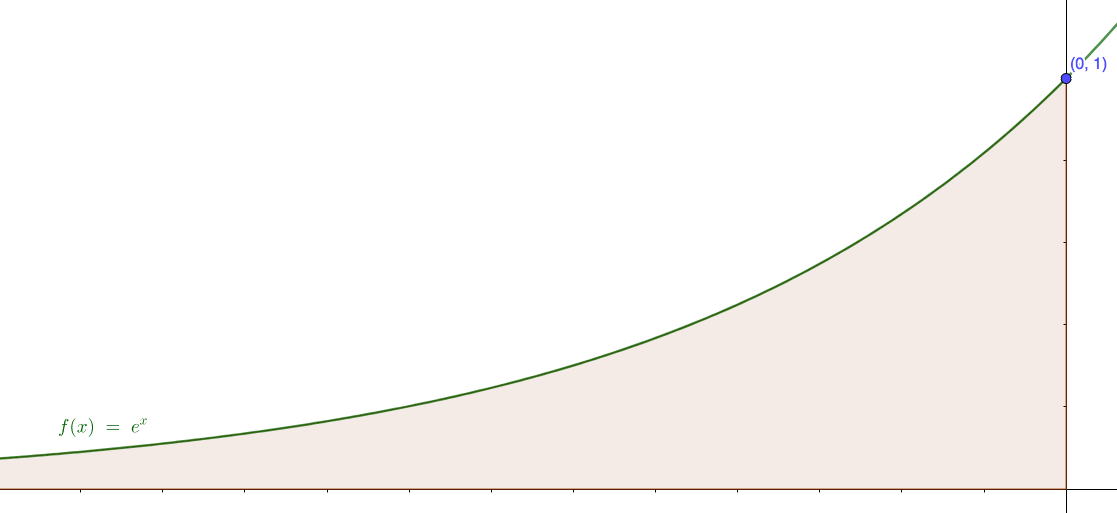
\includegraphics[scale=0.25]{images/e-improper-integral}
\end{ex}
\vspace{-2in}
\begin{thrm}
  Note that \vspace{0.5in} \[
    \hspace{3in} = \int_{-\infty}^c f(x) \dx + \int_c^\infty f(x) \dx
  \]
  for any real number \(c\).
\end{thrm}
%%%%%%%%%%%%%%%%%%%%%%%%%%%%%%%%%%%%%%%%%%%%%%%%%% 
\end{document}
